\documentclass{article}
\usepackage{framed}
\usepackage[letterpaper, margin=1in]{geometry}
\usepackage{graphics}
\usepackage{hyperref}
\usepackage{pgfplots}

\setlength{\parindent}{0pt}
\hypersetup{colorlinks=true, linkcolor=blue, filecolor=magenta, urlcolor=cyan}
\pgfplotsset{compat=1.18}

\title{The Kragle - Battlecode 25 Postmortem}
\author{Justin Ottesen, Andrew Bank, Matt Voynovich}
\date{Last Updated: \today}

\begin{document}

  \maketitle

  \section{Introduction}  

  We believe our postmortem will be of unique help to future Battlecode participants. Often, teams who make postmortems are those who have consistently placed highly from the start. We have the perspective of a team that spent years with no consideration of qualifiers, who this year made the jump to be one of the higher level contenders, going toe-to-toe with the 2 seed in the US qualifiers.

  \medskip

  Hopefully you find this useful!

  \subsection{Our Team - The Kragle}

  We are a team of three computer science students at Rensselaer Polytechnic Institute (RPI). In this year's competition, we made 'the leap' from being a team that couldn't submit a final bot to being a contender for the final tournament. We'll outline some tips and tricks for other aspiring teams to make 'the leap' themselves. We are historically terrible at coming up with team names, and ended up choosing ``The Kragle'' after Justin had a burst of inspiration working on a \verb|MicroManager| class shortly after re-watching The Lego Movie. Just you wait for what we cook up next year. Some more information about us is below:
  
  \medskip

  \textbf{Andrew Bank} has competed in Battlecode since 2021. He is a Computer Science and Computer Systems Engineer at RPI and will graduate in this spring 2025. Andrew has interned at Johns Hopkins Applied Physics Lab, he has created the Circuit Randomizer for Personalized Learning as an undergraduate research project under Professor Shayla Sawyer, and is currently working on another undergraduate research project: the MusicX project for Professor Sawyer's Mercer Xlab. In his free time, Andrew enjoys having more Strava follwers than Instagram followers, and he enjoys treating Stardew Valley like an operating systems optimization problem while playing with his siblings.

  \medskip

  \textbf{Justin Ottesen} has competed in Battlecode since 2022. He began his undergraduate degree in Computer Science in Fall 2021, and graduated early in Spring 2024. He stayed at RPI for his Master's, where he does research with the BRAINS Lab under Oshani Seneviratne with a focus on incentive design for smart contract protocols, and is on track to graduate in Fall 2025. Outside of classwork, he has worked as an intern at Nasuni since Summer 2023, and is on the D3 NCAA Cross Country and Track teams at RPI. In his free time, he enjoys hiking, running, programming, and playing Mario Kart Wii.

  \medskip

  \textbf{Matthew Voynovich} started competing in Battlecode this year. He began his undergraduate degree majoring in both Computer Science and Information Technology and Web Science at RPI in Fall of 2023. He is scheduled to graduate in Spring 2026 and plans to pursue a masters under the Co-Terminal program at RPI. Currently, Matthew works as an undergrad researcher under Thomas Morgan studying quantum phase investigations, and in his free time enjoys long distance running with his friends in the Rensselaer Running Club.

  \newpage
  \subsection{Past Performance}

  Andrew was the only member to compete in 2021. In 2022, Justin joined Andrew, working together again in 2023 and 2024 along with some other teammates. We did not perform particularly well in any of these years, typically holding a 1200-1500 rating, with no notable performances in any of the tournaments. Unfortunately, the RPI spring semester starts very early, so we were always balancing classwork along with the competition. This year we went all in, and entered the US qualifier tournament with the 10 seed, rated at 1730. I guess you'll have read this to see how we did...

  \medskip

  Although we aren't sure our mess of a repository will be useful to anyone else, our GitHub repositories can be found below:
  \begin{enumerate}
    \item[2021] \textbf{Fire Nation} - Lost to the sands of time\dots
    \item[2022] \textbf{Kernel Byters} - \url{https://github.com/justinottesen/Kernel-Byters}
    \item[2023] \textbf{PC Ghosts} - \url{https://github.com/andrewkbank/bc2023} (This is still private)
    \item[2024] \textbf{Goat House} - \url{https://github.com/justinottesen/battlecode24}
    \item[2025] \textbf{The Kragle} - \url{https://github.com/justinottesen/battlecode25} (This is still private)
  \end{enumerate}

  \subsection{Game Overview}

  This year's introduction message is shown below:

  \begin{quote}
    \textit{The bread and food of yore has begun to run out, forcing robot society to adapt. Gone are the jovial ducks, replaced by steampunk robot bunnies who have converted their need for nutrients into a reliance on paint. These bunnies have become territorial, forming clans and defense formations to protect the resource that keeps them running.}
    
    \medskip
    
    \textit{For the past two centuries, these bunnies have stayed within their own territory, but clans have begun to degrade their environment and need to start branching out. Will these clans be able to expand their territory and generate enough paint to protect their families? Or will they stray too close to other clans and be wiped out in conflict?}
  \end{quote}

  As hinted above, this year's game was a competition of territory control between paint-crazy bunnies. The first team to paint 70\% of the map would win. Each team had two starting towers, which could produce robots. These robots had different abilities, but their goal was to work together to build more towers and paint as much territory as possible.

  \subsection{Map}

  The map style was rather simple this year. All maps were within $20 \times 20$ to $60 \times 60$ (inclusive) discrete tiles, and were guaranteed to be either vertically, horizontally, or rotationally symmetrical. Tiles were either empty, walls, or ruins. Robots could move on and paint empty tiles, but they could not for walls and ruins. As always in Battlecode, the map was 

  \subsection{Resources}

  The two resources of this year's game were Money (also referred to as Chips) and Paint.
  
  \medskip

  \textbf{Money} was a globally shared resource and could only be generated through towers. Money could be spent on new towers, tower upgrades, or new robots.
  
  \medskip

  \textbf{Paint} was a more complicated resource to manage, since it was held by individual units. Paint could be produced by towers or stolen from enemies, and could be spent to attack, expand territory, or produce new robots. When painted on the map, paint could be either a primary or secondary color for each team, and this was used to designate special patterns, which are described further below.

  \subsection{Towers}

  There were three tower types: Money towers, Paint towers, and Defense towers. Money and Paint towers passively produced their respective resources, and Defense towers initially just had high attack and health, but were buffed to also produce chips on every attack.

  \medskip

  Towers could do a weak attack to all enemies in their attack radius, and a stronger attack to a single enemy per turn. Towers could only be constructed at sites on the map called Ruins. Each tower type had its own $5 \times 5$ pattern that needed to be painted around a ruin before a tower could be built there. In addition, teams were limited to 25 towers at any given time.

  \subsection{Robots}

  There were three robot types: Soldiers, Splashers, and Moppers.

  \medskip

  \textbf{Soldiers} were the ``standard'' unit of this year. They could paint tiles to a team's color or attack enemy towers. Importantly, soldiers could not paint over enemy paint. They could only paint empty tiles, or allied tiles (which was useful in painting a pattern).

  \medskip

  \textbf{Splashers} could paint a group of tiles, regardless of their current paint status. However, they were more expensive than soldiers, and their attack was far less paint efficient. This attack also damaged enemy towers in range.

  \medskip

  \textbf{Moppers} could remove enemy paint from tiles. If an enemy was on the tile, it would also steal some of their paint and give it to the mopper. They also had the ability to swing their mop, which could attack close-by groups of clustered enemies, taking away enemy paint.

  \subsection{Special Resource Patterns}

  In addition to the tower patterns that could be painted on the map, robots could paint Special Resource Patterns (SRPs), which boosted the production rate of all friendly towers. A balance change caused these to have a 200 chip cost to complete, and would only activate after being completed for 50 consecutive turns. As soon as the pattern was disturbed, it would be deactivated.

  \subsection{Communication}

  Communication was relatively restricted this year. Robots could not communicate with each other, they could only communicate by messaging towers when they were close by and there was a path of friendly paint connecting them. Towers could send messages to robots and they could broadcast messaged to other towers within a slightly larger range. Robots could only send one message per round, and towers could send 20. The message consisted of the round number, the sending robot ID, and a 32 bit integer.

  \medskip

  The other simpler way of communicating is that robots can mark a 1 or a 2 on any empty tile. This is intended for robots to let others know what color tiles should be painted, but it can also be used for very simple communication.

  \section{Strategy \& Implementation}

  \subsection{Sprint 1}

  \subsubsection{Setup}

  The first thing we did was decide how to structure our code. We took a lot of inspiration from XSquare's 2024 code \url{https://github.com/IvanGeffner/BTC24}. We created an abstract \verb|Robot| class, and created a subclass for each robot type (\verb|Soldier|, \verb|Splasher|, \verb|Mopper|, \verb|Tower|). This heavily simplified our \verb|RobotPlayer| class, and helped us split functionality between differing robot types\footnote{In hindsight, it may have been even smarter to have another level to the hierarchy where we had Unit as the base class, Robot and Tower as subclasses, and other types inherit from these. Towers don't need to do pathfinding, and they can't really learn much about the map, so this was bad organization and wasted bytecode}. Along with these classes, we also had utility classes, like \verb|MapData|, \verb|Explore|, \verb|Bugpath|, and others.

  \medskip

  Our first priority was getting a bot that could effectively explore and capture towers. This was our first priority since building towers would allow our team to increase their resource income and create more robots. We had each tower spawn a soldier and a mopper who would search for a ruin. We copied the capture logic from examplefuncsplayer. The soldier was to paint the pattern around the tower, and the mopper was to clear any enemy paint in the way.

  \subsubsection{Resources \& Towers}

  We made two observations very early on about resources:
  \begin{enumerate}
    \item It is not worth upgrading towers.
    \item It Money towers are always better than Paint towers.
  \end{enumerate}
  The first one is relatively obvious looking at the costs of new towers vs upgrades. For Money towers, the following table shows the cost associated with each level of the tower:
  \begin{center}
    \begin{tabular}{c | c | c}
      Level & Upgrade Cost (Chips) & Mining Rate (Chips / Turn) \\
      \hline 
      1 & 1000 & 20   \\
      2 & 2500 & 30   \\
      3 & 5000 & 40   \\
    \end{tabular}
  \end{center}
  From this table, we can graph the cost and mining rates:
  \begin{center}
    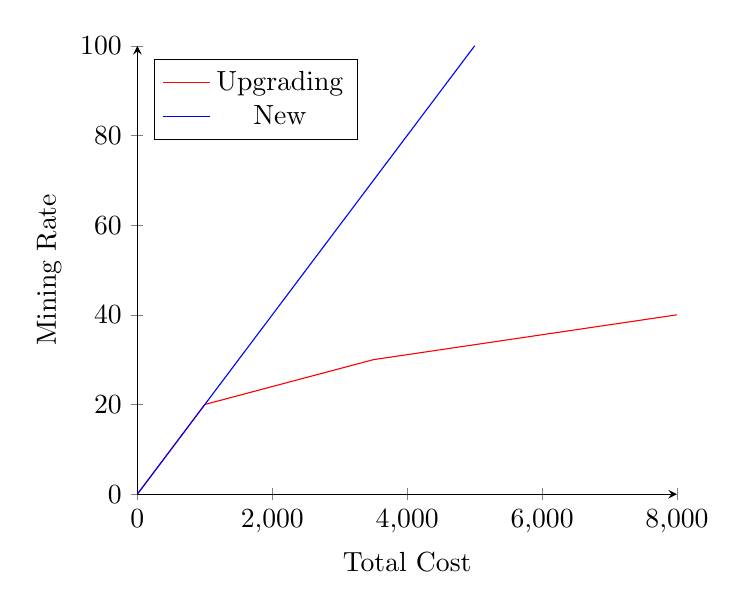
\begin{tikzpicture}
      \begin{axis}[
        axis lines = left,
        xlabel = Total Cost,
        ylabel = Mining Rate,
        legend pos = north west
      ]
      \addplot [
        color = red
      ]
      coordinates {
        (0,0)(1000,20)(3500,30)(8000,40)
      };
      \addlegendentry{Upgrading}

      \addplot [
        color = blue,
        domain = 0:5000
      ]
      { x / 50 };
      \addlegendentry{New}
        
      \end{axis}
    \end{tikzpicture}
  \end{center}
  As is clearly shown here, when you have the choice between spending on a new tower, or upgrading an existing one, there is no reason to upgrade. The same can be said for Paint towers, but the next observation makes that redundant.

  \medskip

  Even though paint is arguably the more important resource, Paint towers are useless\footnote{This is true until you factor in SRPs, but we are getting there} because money towers actually produce paint more effectively than paint towers. Each tower spawns with 500 paint. Since money towers produce 20 chips per turn and they cost 1,000 chips, they pay for themselves in 50 turns. So, if a Money tower calls \verb|rc.disintegrate()|, we can trade 1,000 chips for 500 paint. If we do this every 50 turns, money towers have an effective paint mining rate of 10 paint per turn, which is double what paint towers are capable of.

  \medskip

  Here is the corresponding graph to the above for paint production vs chip cost:
  \begin{center}
    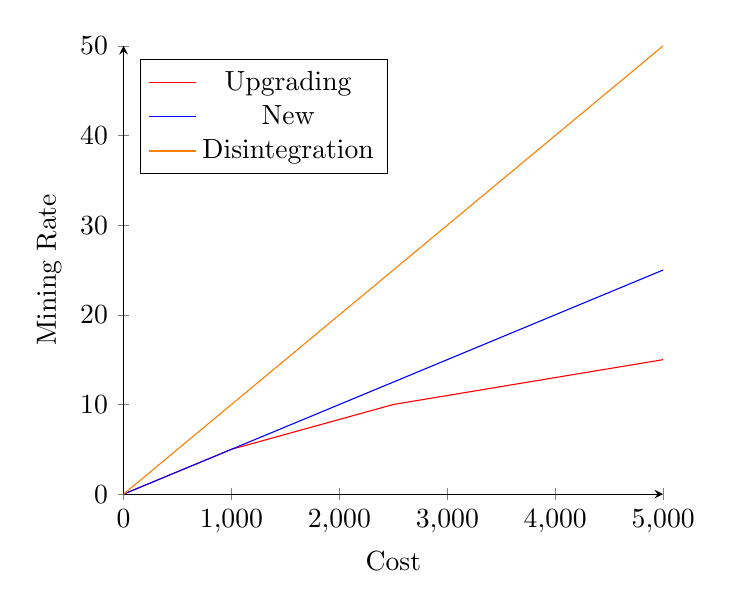
\begin{tikzpicture}
      \begin{axis}[
        axis lines = left,
        xlabel = Cost,
        ylabel = Mining Rate,
        legend pos = north west
      ]
      \addplot [
        color = red
      ]
      coordinates {
        (0,0)(1000,5)(2500,10)(5000,15)
      };
      \addlegendentry{Upgrading}

      \addplot [
        color = blue,
        domain = 0:5000
      ]
      { x / 200 };
      \addlegendentry{New}
      
      \addplot [
        color = orange,
        domain = 0:5000
      ]
      { x / 100 };
      \addlegendentry{Disintegration}
      \end{axis}
    \end{tikzpicture}
  \end{center}
  There are a few other big bonuses of this strategy:
  \begin{enumerate}
    \item We now have the choice of converting chips to paint. With paint towers, if we have more paint than we need or can use, we are stuck with it.
    \item We no longer have to coordinate what tower types we are building, since we are always building money towers (we ignore defense towers for now).
    \item Since chips are global and paint is local, we can use money towers that are far away from the active parts of the map to subsidize tower production where it is needed most.
  \end{enumerate}

  \subsubsection{Special Resource Patterns}

  However, once SRPs are introduced, this math changes. Each active SRP boosts paint production by 3 units per tower per turn. The following table shows how the number of SRPs affects the per turn production rates of different towers:
  \begin{center}
    \begin{tabular}{c | c | c | c}
      SRPs & Money Tower Chips & Money Tower Paint\footnote{This represents the amount of paint which can be effectively achieved per turn by disintegrating and rebuilding money towers} & Paint Tower Paint \\
      \hline
      0 & 20 & 10 & 5 \\
      1 & 23 & 11.5 & 8 \\
      2 & 26 & 13 & 11 \\
      3 & 29 & 14.5 & 14 \\
      4 & 32 & 16 & 17 \\
      5 & 35 & 17.5 & 20
    \end{tabular}
  \end{center}
  As you can see, once there are 4 or more SRPs, paint towers are better suited for their intended purpose. We decided not to worry about this and stick with our money tower only strategy, to keep things simple for Sprint 1. Plus, we (regrettably) did not prioritize SRPs for Sprint 1, our soldiers simply checked if the current location could have an SRP and if so, they marked one.

  \subsubsection{Pathfinding \& Map Representation}

  Units stored their knowledge of the map in memory, however we ended up rewriting this system, so this will be described further later. Units traversed the map using a BugNav algorithm. We reused an algorithm from XSquare \url{https://github.com/IvanGeffner/BTC24/blob/master/BugPath.java}, and it worked with minor tweaking. If you have questions about how this works, there was a lecture on it this year \href{https://www.youtube.com/live/Mqk50BQH3oQ?si=6qL5WAXmSOS2K3OR}{here}.\\
  Pathfinding wasn't a high priority this year since ruins/towers guaranteed a lot of open space. In theory, Teh Devs could've made maps with few ruins and many walls, but that never happened. Even though something like unrolled BFS would've been optimal, BugNave worked well enough in practice, and because source code for it already existed, we saved a lot of time not worrying about pathfinding.
  
  \subsubsection{Sprint 1 Performance}

  We entered the tournament as the 55 seed out of 160 teams, with a rating of 1533, our first match was a 4-1 win against the 74 seed, ``be right back'' with a rating of 1483. Their strategy was to do an early rush with soldiers to try and take out our towers, then produce a single splasher to cover some paint. This worked against us on the first game, as our starting soldiers got stuck trying to capture an SRP with enemy paint, and our moppers didn't help them.

  \medskip

  The left image below shows the result of our loss, and the right image shows one of our wins. On this particular map, the opponent's rush got trapped against a wall, 
  \begin{center}
    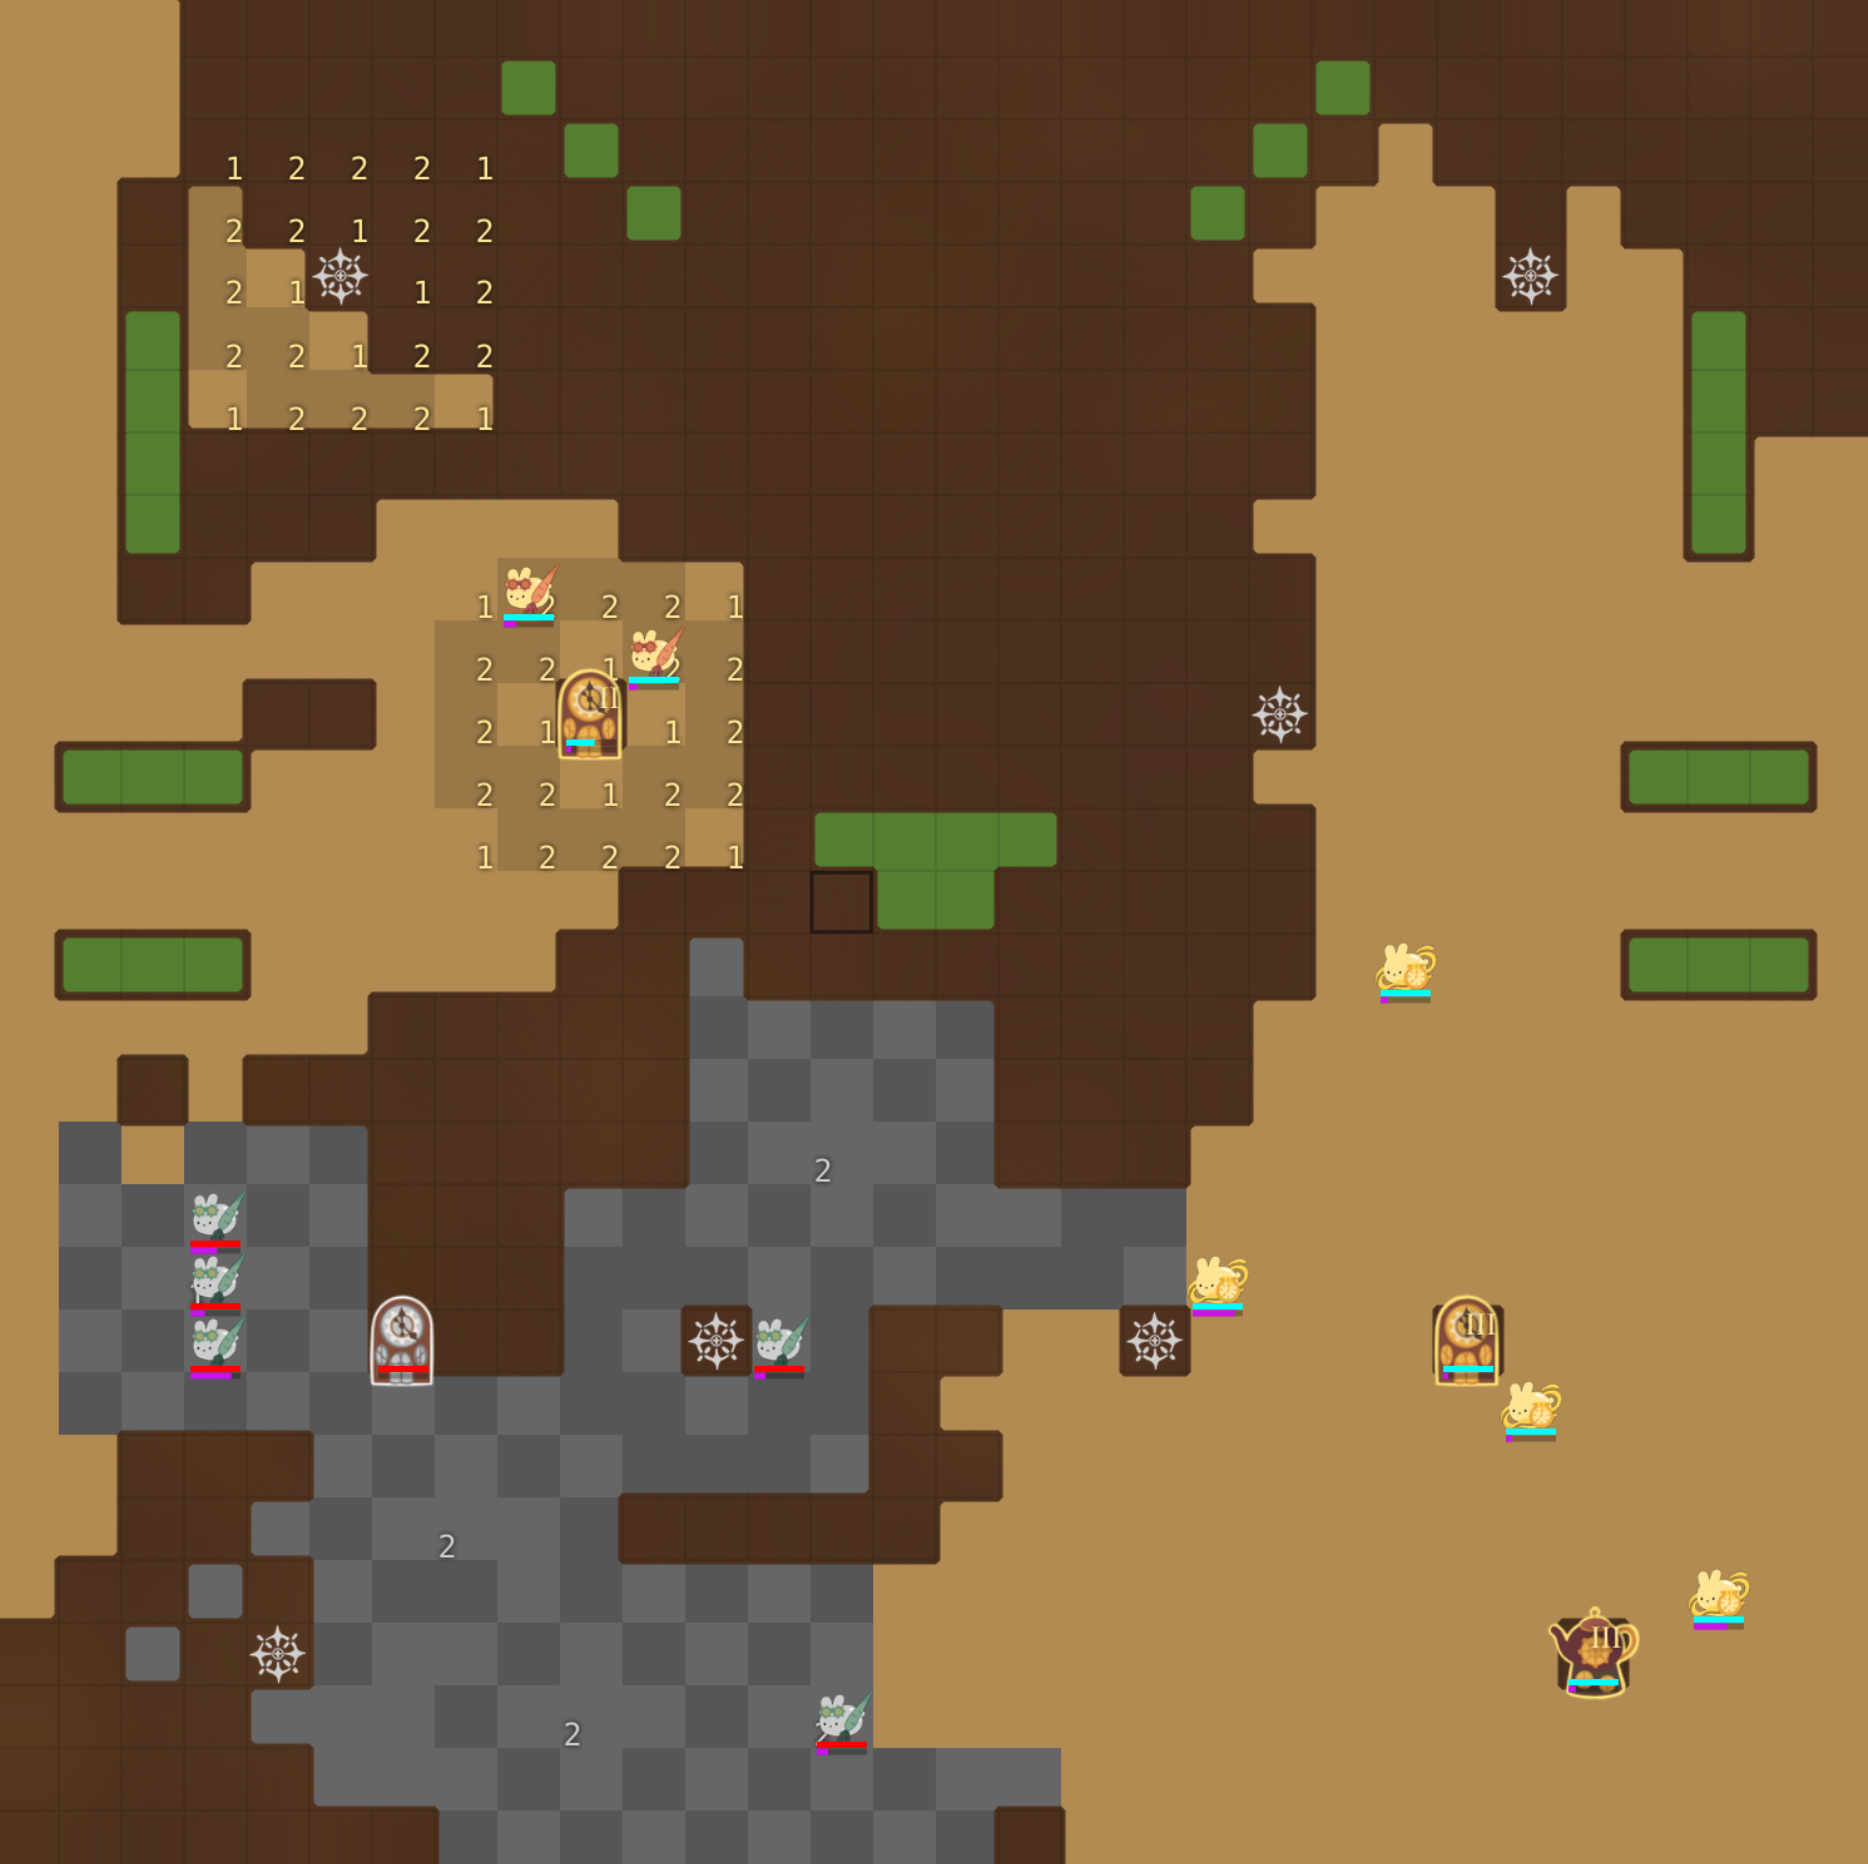
\includegraphics[scale=0.1]{images/sprint1_loss.png}
    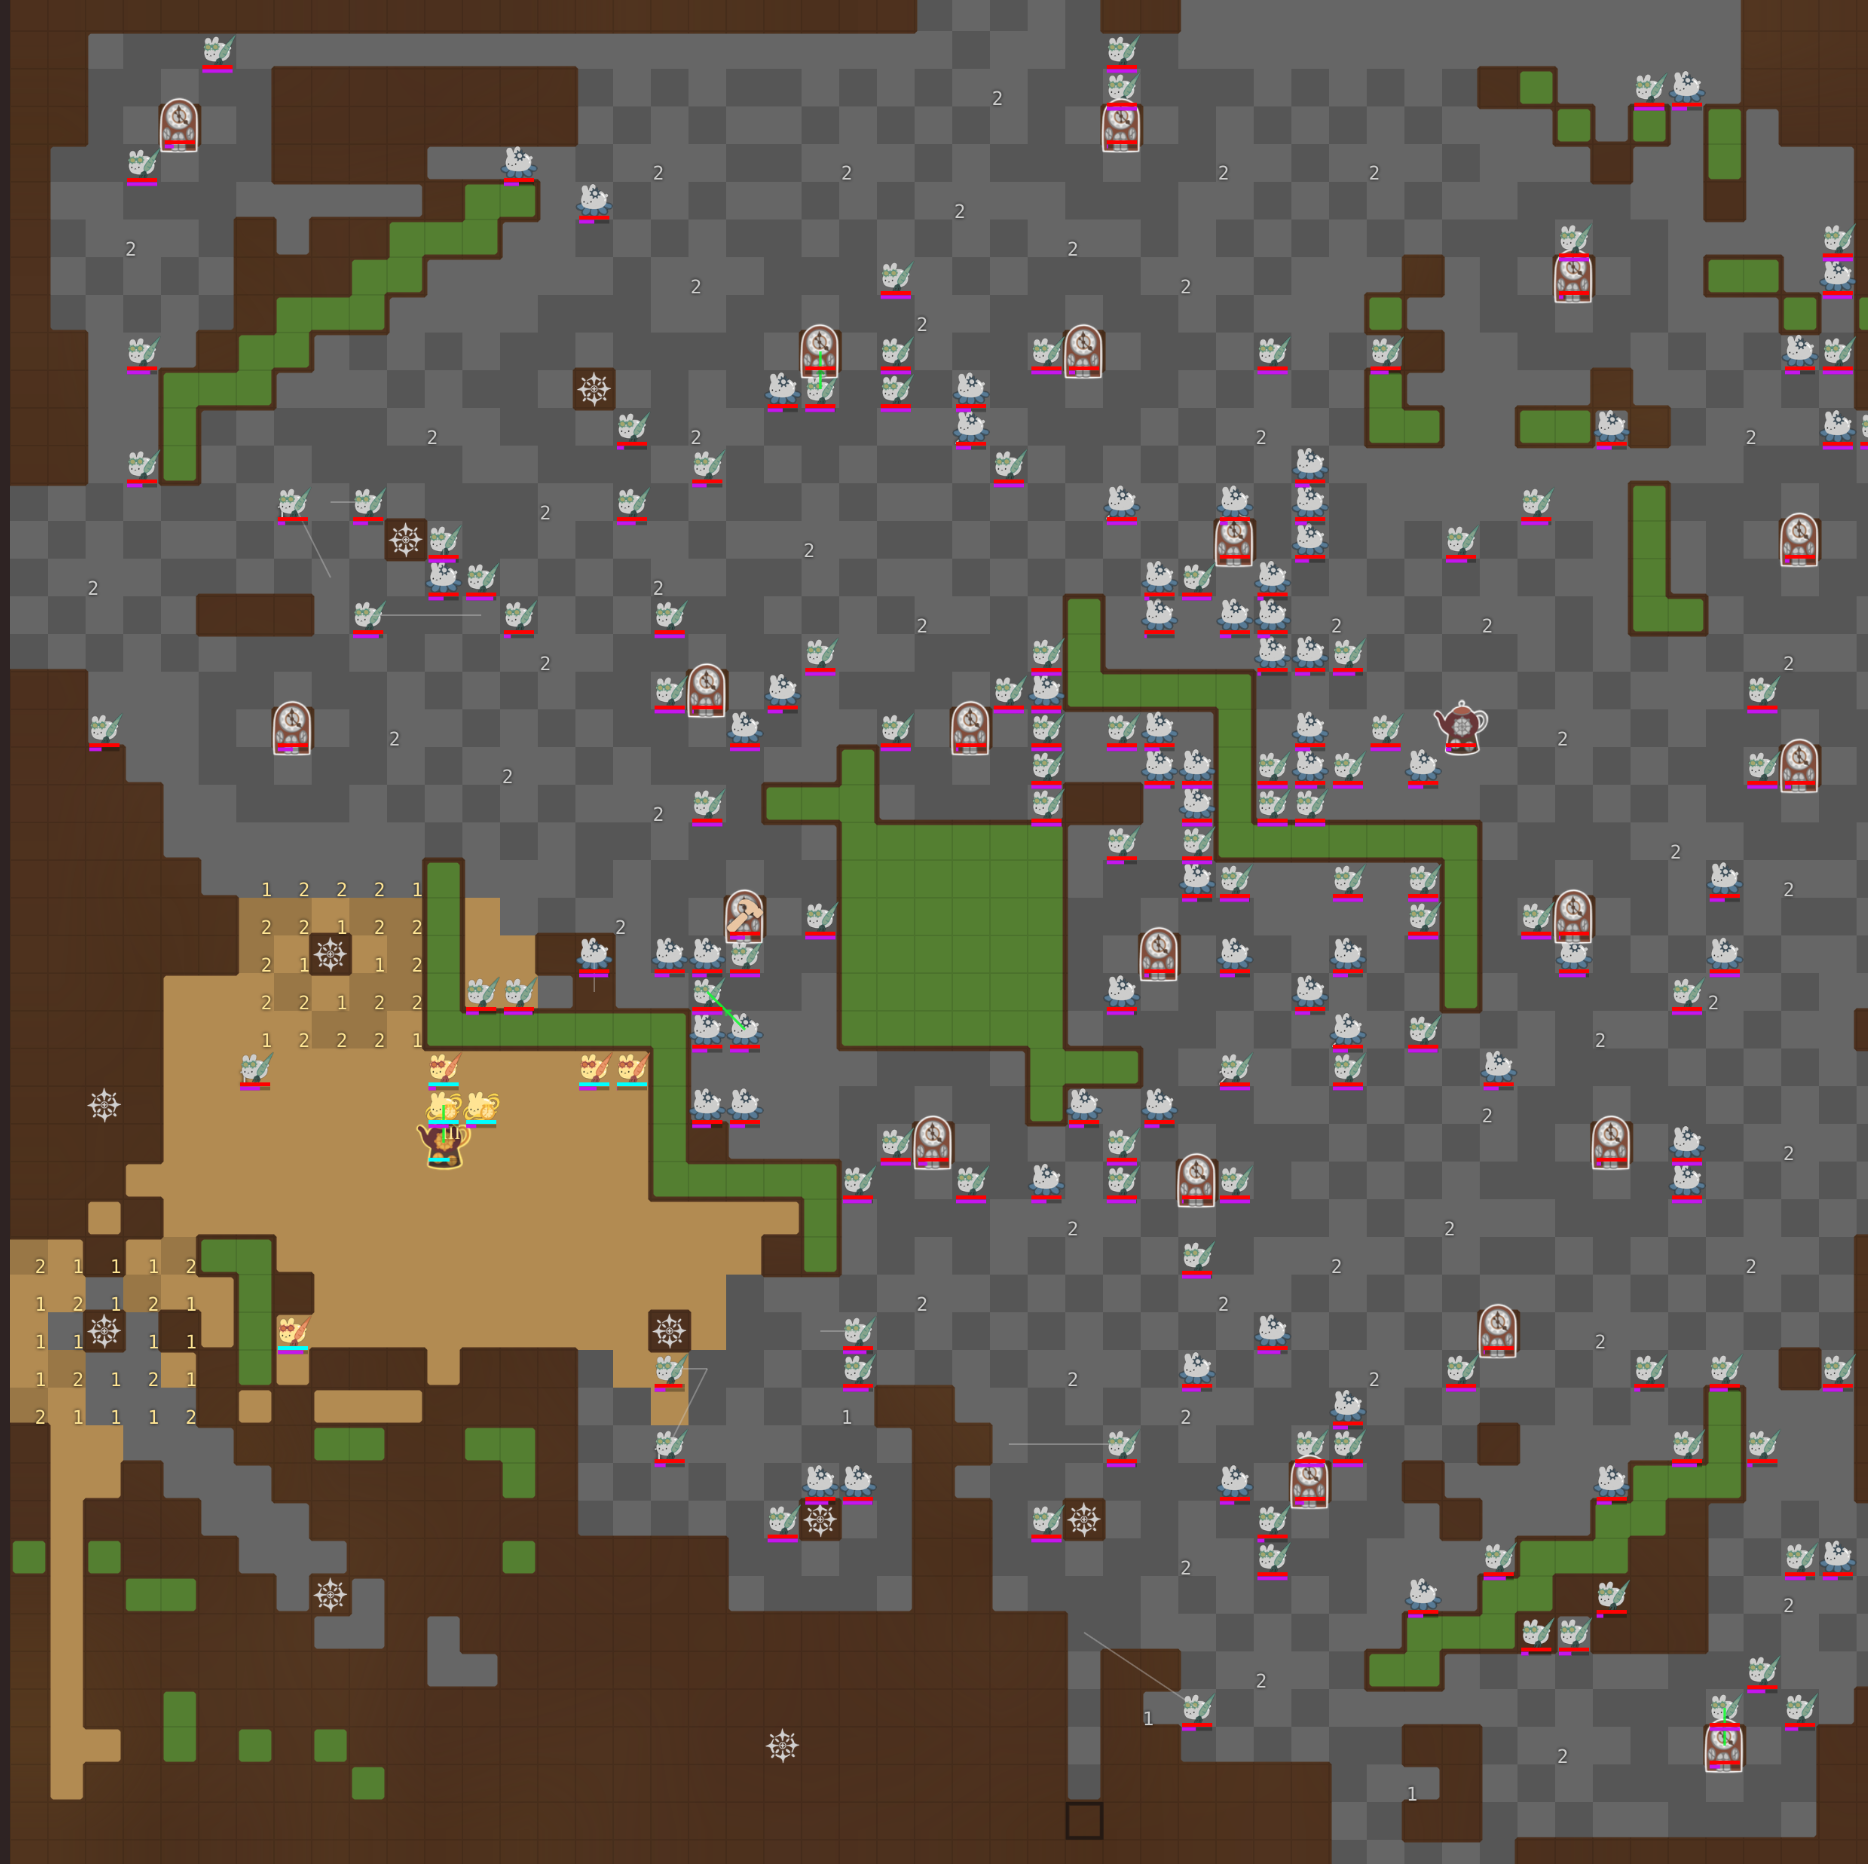
\includegraphics[scale=0.1]{images/sprint1_win.png}
  \end{center}

\end{document}